\chapter{FISSA -- Fault Injection Simulation for Security Assessment}
\chaptermark{FISSA - Fault Injection Simulation for Security Assessment}
\label{chapter:fissa}
\minitoc

This section introduces and presents a tool, called FISSA -- Fault Injection Simulation for Security Assessment --, created to automate fault injection attacks campaigns in simulation. The first section presents the state of the art of existing tools for FIA campaigns in emulation, formal methods or even perform real world attacks. The second section presents the architecture and details how FISSA works and presents how to extend it depending on other needs. Finally, we will discuss and draw some perspectives for the tool's development and usability.

%%%%%%%%%%%%%%%%%%%%%%%%%%%%%%%%%%%%%%%%%%%%%%%%%%%%%%%%%%%%%%%%%%%%%%%%%%%%%%%%%%%%%%%%%%%%%%%
\section{Simulation tools for Fault Injection}
This section presents recent works related to methods and tools for vulnerability assessment when considering fault injection attacks. For such vulnerability assessment, main strategies include actual fault injections, emulations, formal methods and simulations.

\begin{table}[t]
    \centering
    \caption{Fault Injection based methods for vulnerability assessment comparison}
    \label{table:FI_type_comparison}
    \normalsize
    \setlength{\tabcolsep}{1pt}
    \begin{tabular}{@{}lccccccc@{}}
        \toprule
                          & References  & Cost                                & \begin{tabular}[c]{@{}c@{}}Control over\\fault scenarios\end{tabular}       & Scalability                         & Speed of execution                                      & Realism                             & Expertise \\ \midrule
        Formal Methods    & \cite{BSSMG-21-tchess, ANR-18-ices, BBCFGS-19-esorics, SVPMRDKMS-24-eprint}     & \textcolor{ForestGreen}{Very low}  & \textcolor{ForestGreen}{Very high}  & \textcolor{red}{Very low}           & \textcolor{red}{Low}                                    & \textcolor{red}{Low}                & \textcolor{red}{Very high} \\
        Simulations  & \cite{AB-23-acns, fisim, AWMN-20-host}     & \textcolor{ForestGreen}{Very low}       & \textcolor{ForestGreen}{Very high}  & \textcolor{red}{Low}                & \textcolor{red}{Low}/\textcolor{ForestGreen}{Moderate}  & \textcolor{ForestGreen}{Moderate}   & \textcolor{ForestGreen}{Low} \\
        Emulations        & \cite{CMLCVR-11-crypto, HGASO-21-fdtc,BLK-23-access, NNHRS-14-dsd}     & \textcolor{Red}{High}           & \textcolor{ForestGreen}{Moderate}   & \textcolor{ForestGreen}{High}  & \textcolor{ForestGreen}{Very high}                      & \textcolor{ForestGreen}{High}       & \textcolor{red}{Moderate} \\
        Actual FIA        & \cite{BCNTW-06-procieee, BFP-19-tches, GBD-23-paine, CGVCBLC-22-cardis}     & \textcolor{Red}{Very high}           & \textcolor{Red}{Very low}           & \textcolor{ForestGreen}{Very high}  & \textcolor{ForestGreen}{Very high}                      & \textcolor{ForestGreen}{Very high}  & \textcolor{red}{Very high} \\
        \bottomrule
    \end{tabular}
\end{table}

Actual FIAs involve physically injecting faults into the target hardware using techniques such as variations in supply voltage or clock signal~\cite{BCNTW-06-procieee, BFP-19-tches}, laser pulses~\cite{BCNTW-06-procieee, CGVCBLC-22-cardis}, electromagnetic emanations~\cite{BCNTW-06-procieee} or X-Rays~\cite{GBD-23-paine}.
This approach offers valuable insights into the real impact of faults on hardware components.
However, a significant drawback of actual fault injections is that they demand considerable expertise to prepare the target, involving intricate setup procedures.
Additionally, this approach can only be executed once the physical circuit is available, potentially delaying the vulnerability assessment process until later stages of development.


Fault emulation can, for instance, rely on FPGA~\cite{CMLCVR-11-crypto}, or on an emulator such as QEMU~\cite{HGASO-21-fdtc,BLK-23-access} to perform fault injection campaigns. This approach is four times faster than simulation-based techniques~\cite{NNHRS-14-dsd}, and unlike simulation-based or formal method-based fault injections techniques, the size of the evaluated circuit has no major impact on the fault injection campaign timing performances.
However, configuring an emulation environment can be complex and time-consuming. Achieving an accurate representation of the target system may require detailed configuration and parameter tuning. The accuracy of emulation is contingent on the quality of the models used to replicate the target hardware. If the models are inaccurate or incomplete, the results of fault injections may not precisely reflect actual behaviour.

Formal methods provide an advantage with mathematical proofs, ensuring a rigorous verification of the system's behaviour during fault injection experiments. Formal methods approaches such as~\cite{BSSMG-21-tchess} allow the analysis of a circuit design in order to detect sensitive logic or sequential hardware elements. \cite{ANR-18-ices}, \cite{BBCFGS-19-esorics} and~\cite{SVPMRDKMS-24-eprint} present formal verification methods to analyse the behaviour of HDL implementation.
However, this type of tool usually suffers from restrictions limiting its actual usage on a complete processor.
Conventional formal approaches encounter scalability challenges due to limitations in verification techniques.
In particular, the circuit structure it can analyse is usually limited.

Fault Injections simulations can be performed at processor instructions level. Authors of~\cite{AB-23-acns} explore the impact of fault injection attacks on software security. They evaluate four open-source fault simulators, comparing their techniques and suggest enhancing them with AI methods inspired by advances in cryptographic fault simulation. \cite{fisim} is an open-source deterministic fault attack simulator prototype utilising the Unicorn Framework and Capstone disassembler.
\cite{AWMN-20-host} introduces VerFI, a gate-level granularity fault simulator for hardware implementations. For instance, it has been used to spot an implementation mistake in ParTI~\cite{SMG-16-crypto}.
However, this tool has been developed to check if implemented countermeasures can really protect against fault injection on cryptographic implementations, but it cannot evaluate components such as registers or memories.
In this paper, we focus on Cycle Accurate Bit Accurate (CABA) Simulation, which provides a controlled virtual environment for injecting faults. There are several solutions of simulations in an HDL simulator like Questasim, Vivado, etc. \textit{Behavioural} simulation is used to detect functional issues and ensuring that the design behaves as expected. \textit{Post-synthesis} simulation verifies that the synthesised netlist matches the expected functionality. \textit{Timed} simulation is used to ensure that the design meets timing requirements and can operate at the specified clock frequency. And finally, \textit{post-implementation} simulations are used to verify that the implemented design meets all requirements and constraints, including those related to the physical layout on the target.
Simulation-based fault injection offers the advantage of enabling designers to test their system throughout the design cycle, providing valuable insights and uncovering potential vulnerabilities early in the development process. However, a limitation lies in the potential lack of absolute fidelity to actual conditions, as simulations might not perfectly replicate all hardware intricacies, introducing a slight risk of overlooking certain faults that could manifest in the actual hardware.

Table~\ref{table:FI_type_comparison} shows a comparison between these four methods for vulnerability assessment when considering FIA regarding six metrics. These metrics are the financial cost of setting up the fault injection campaign, the control over fault scenarios (how configurable are the scenarios), scalability which refers to the method capacity to be applied to systems of different sizes or complexities, speed of execution of the campaign, realism of the fault injection campaign and the level of required expertise.
Table~\ref{table:FI_type_comparison} shows that no method is completely optimal. Each method has its own advantages and disadvantages and must be chosen by the designer according to the requirements and the available financial and human resources. Indeed, setting up an actual fault injection campaign requires much more expertise in this domain and also requires costly equipment, whereas setting up a simulation campaign can be easier for a circuit designer familiar with HDL simulation tools such as Questasim.
Table~\ref{table:FI_type_comparison} shows that CABA simulation offers a good compromise to assess the security level of a circuit design. In particular, it provides an efficient solution for investigating security throughout the design cycle, enabling the concept of “Security by Design”.

%%%%%%%%%%%%%%%%%%%%%%%%%%%%%%%%%%%%%%%%%%%%%%%%%%%%%%%%%%%%%%%%%%%%%%%%%%%%%%%%%%%%%%%%%%%%%%%
\section{FISSA}
This section presents our open-source tool, FISSA~\cite{fissa}. It is under the CeCILL-B licence and available on GitHub.

\subsection{Main software architecture}
FISSA is designed to help circuit designers to analyse, throughout the design cycle, the sensitivity to FIA of the developed circuit.
Figure~\ref{fig:archi_fissa} presents the software architecture of FISSA.
It consists of 3 different modules: \textit{TCL generator}, \textit{Fault Injection Simulator} and \textit{Analyser}. The first and third modules correspond to a set of Python classes.
\textit{The TCL generator}, detailed in Section~\ref{subsec:tcl_gen}, relies on a configuration file and a target file to create a set of parameterised TCL scripts. These scripts are tailored based on the provided configuration file and are used to drive the fault injection simulation campaign.

\textit{Fault Injection Simulator}, detailed in Section~\ref{subsec:FIS}, performs the fault injection simulation campaign based on inputs files from \textit{TCL generator} for a circuit design described through HDL files and memory initialisation files. For that purpose it relies on an existing HDL simulator such as Questasim~\cite{questasim}, Verilator~\cite{verilator}, or Vivado~\cite{vivado}.

\textit{The Analyser}, detailed in Section~\ref{subsec:analyser}, evaluates the outcomes of the simulations and generates a set of files that allows the designers to examine fault injection effects on their designs through various information.


\begin{figure}[ht]
    \centering
    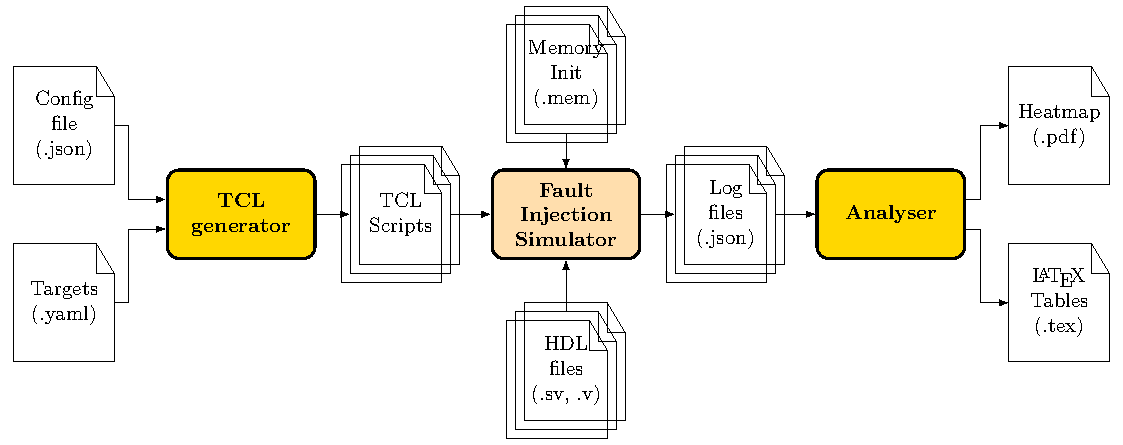
\includegraphics[width=\textwidth]{c4_fissa/img/fissa/archi_gen_tcl.pdf}
    \caption{Software architecture of FISSA}
    \label{fig:archi_fissa}
\end{figure}

Algorithm~\ref{algo:pseudoCodeSimuStages} shows a representation of a fault injection campaign. The algorithm requires a set of targets  (i.e. hardware elements in which a fault should be
injected), the fault model and the considered injection window(s) which identifies the period(s), in number of clock cycles, in which fault injections are performed.
Then, it runs a first simulation with no fault injected, which is used as a reference for comparison with the following simulations to determine end-of-simulation statuses. 
Then, for each target, each fault model and for each clock cycle within the injection window, the corresponding simulation is executed, and the corresponding logs are stored in a dedicated file.

Customising end-of-simulation statuses allows for adaptation to the specific requirements of each design assessment. To configure these statuses, adjustments need to be made either directly in FISSA's code or the HDL code. This process may involve evaluating factors such as:
\begin{itemize}
    \item hardware element content (signal, registers, \ldots),
    \item simulation time (e.g. the simulation exceeds a reference number of clock cycles),
    \item simulation's end (e.g. an assert statement introduced in the HDL code is reached)
\end{itemize}

\begin{algorithm}
    \caption{Simulated FIA campaign pseudo-code}
    \label{algo:pseudoCodeSimuStages}
    \normalsize
    \begin{algorithmic}[1]
        \Require $targets \leftarrow list(targets)$
        \Require $faults \leftarrow list(fault_model)$
        \Require $windows \leftarrow list(injection_windows)$
            \State $ref_sims = simulate()$
            \For{$target \in targets$}
                \For{$fault \in faults$}
                    \For{$cycle \in windows$}
                        \State $logs = simulate(target, fault, cycle)$
                    \EndFor
                \EndFor
            \EndFor
    \end{algorithmic}
\end{algorithm}

\subsection{Supported fault models}
\label{subsec:supported_fault_models}

A set of fault models has already been integrated into FISSA. For a given fault injection campaign, the relevant fault model is defined in the input configuration file and is applied to targets during the simulation phase.
Currently, supported fault models are:
\begin{itemize}
    \justifying
    \item target set to 0/1,
    \item single bit-flip in one target at a given clock cycle,
    \item single bit-flip in two targets at a given clock cycle,
    \item single bit-flip in two targets at two different clock cycles,
    \item exhaustive multi-bits faults in one target at a given clock cycle,
    \item exhaustive multi-bits faults in two targets at a given clock cycle.
\end{itemize}

\subsection{TCL Generator}
\label{subsec:tcl_gen}

The \textit{TCL Generator} is used to generate the set of TCL script files which drive the \textit{fault injection simulator}. This module requires two input files.
Figure~\ref{fig:archi-scriptGen} details the \textit{TCL Generator}. Each blue box represents a python class used to generate the set of output TCL scripts.
The initialisation class gets inputs from a configuration file. This JSON-formatted file includes various parameters such as the targeted HDL simulator, the considered fault model and the injection window(s). Furthermore, it encompasses parameters such as the clock period (in ns) of the HDL design and the maximum number of simulated clock cycles used to stop the simulation in case of divergence due to the injected fault. Moreover, one extra parameter defines the quantity of simulations per TCL file, allowing a simulation parallelism degree.
The \textit{Targets} file contains, in YAML format, the list of the circuit elements (e.g. registers or logic gates) that need to be targeted during the fault injection campaign. For each target, its HDL path and bit-width are specified.
\textit{TCL Script Generator} class gets the configuration parameters from \textit{Initialisation} class, reads the \textit{Targets'} file and calls three others classes.
The first one, \textit{Basic Code Generator}, undertakes the fundamental generation of TCL code for initialising a simulation, running a simulation, and ending a simulation.
The second one, \textit{Fault Generator}, produces the TCL code related to fault injection. The \textit{TCL Script Generator} provides specific parameters to the \textit{Fault Generator} to produce code for a designated set of targets and a specified set of clock cycles for fault injection.
The third one, \textit{Log Generator}, produces the TCL code to produce logs after each simulation.
Logs comprise the simulation's ID, fault model, faulted targets, injection clock cycle(s), end-of-simulation status, values for all targets, and the end-of-simulation clock cycle. This data constitutes the automated aspect of logging.
Finally, the \textit{TCL Script Generator} outputs a set of TCL files, each one correspond to a batch of simulations. It is worth noting that each batch starts with a reference simulation (i.e. without fault injection). This allows the user to perform a per batch results analysis.
Furthermore, it produces a target file used by TCL scripts to get the target list (see Subsection~\ref{subsec:FIS}).

\begin{figure}[ht]
    \centering
    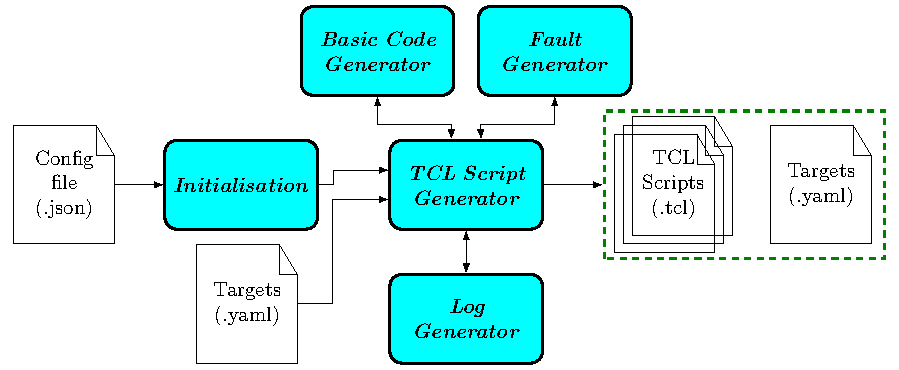
\includegraphics[width=\textwidth]{c4_fissa/img/fissa/detail_tcl_gen.pdf}
    \caption{Software architecture of the TCL Generator module}
    \label{fig:archi_tcl_gen}
\end{figure}

Algorithm~\ref{algo:pseudoCodeSimus} depicts a fault injection simulation pseudo-code, showcasing requirements, each state with essential parameters, and the corresponding Python class from Figure~\ref{fig:archi_tcl_gen}.
Line 5 in Algorithm~\ref{algo:pseudoCodeSimuStages} corresponds to Algorithm~\ref{algo:pseudoCodeSimus}. This algorithm is executed multiple times with different inputs to build a TCL script.


\begin{algorithm}
    \caption{FIA simulation pseudo-code}
    \label{algo:pseudoCodeSimus}
    \normalsize
    \begin{algorithmic}[1]
        \Require $target$
        \Require $cycle$
        \Require $fault_model$
        \State $tcl_script = init_sim(fault_model, cycle, target)$ \textcolor{blue}{\scriptsize // generated by Basic Code Generator}
        \State $tcl_script += inject_fault(fault_model)$  \textcolor{red}{\scriptsize // generated by Fault Generator}
        \State $tcl_script += run_sim()$ \textcolor{blue}{\scriptsize // generated by Basic Code Generator}
        \State $tcl_script += log_sim(fault_model)$ \textcolor{ForestGreen}{\scriptsize // generated by Log Generator}
        \State $tcl_script += end_sim()$ \textcolor{blue}{\scriptsize // generated by Basic Code Generator}
        \State $tcl_file.write(tcl_script)$
    \end{algorithmic}
\end{algorithm}

\subsection{Fault Injection Simulator}
\label{subsec:FIS}

\subsection{Analyser}
\label{subsec:analyser}

\subsection{Extending FISSA}

%%%%%%%%%%%%%%%%%%%%%%%%%%%%%%%%%%%%%%%%%%%%%%%%%%%%%%%%%%%%%%%%%%%%%%%%%%%%%%%%%%%%%%%%%%%%%%%
\section{Discussion and Perspectives}

%%%%%%%%%%%%%%%%%%%%%%%%%%%%%%%%%%%%%%%%%%%%%%%%%%%%%%%%%%%%%%%%%%%%%%%%%%%%%%%%%%%%%%%%%%%%%%%
\section{Summary}

%%%%%%%%%%%%%%%%%%%%%%%%%%%%%%%%%%%%%%%%%%%%%%%%%%%%%%%%%%%%%%%%%%%%%%%%%%%%%%%%%%%%%%%%%%%%%%%